\documentclass[10pt]{standalone}
\usepackage[utf8]{inputenc}
\usepackage{pgf,tikz,pgfplots}
\pgfplotsset{compat=1.15}
\usepackage{mathrsfs}
\usetikzlibrary{arrows}
\pagestyle{empty}
\begin{document}

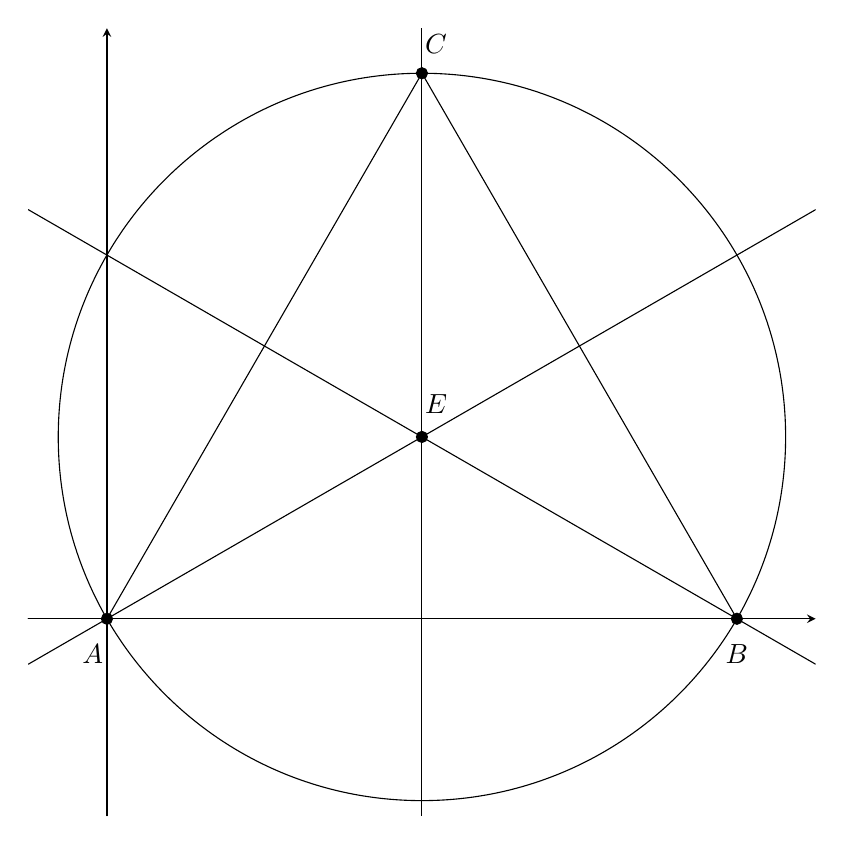
\begin{tikzpicture}[line cap=round,line join=round,>=triangle 45,x=1.0cm,y=1.0cm]
\begin{axis}[
x=1.0cm,y=1.0cm,
axis lines=middle,
%ymajorgrids=true,
%xmajorgrids=true,
xmin=-1.0,
xmax=9.0,
ymin=-2.5,
ymax=7.5,
ticks=none]
\clip(-1.,-2.5) rectangle (9.,7.5);
%\fill[color=black,fill=black,fill opacity=0.1] (0.,0.) -- (8.,0.) -- (4.,6.928203230275509) -- cycle;
\draw  (0.,0.)-- (8.,0.);
\draw  (8.,0.)-- (4.,6.928203230275509);
\draw  (4.,6.928203230275509)-- (0.,0.);
\draw  (4.,2.3094010767585025) circle [radius=4.618802153517006cm];
\draw [domain=-1.:9.] plot(\x,{(--32.-4.*\x)/6.928203230275509});
\draw [domain=-1.:9.] plot(\x,{(-0.-4.*\x)/-6.928203230275509});
\draw  (4.,-2.5) -- (4.,7.5);
\begin{scriptsize}
\draw [fill=black] (0.,0.) circle [radius=2.0pt];
\draw (-0.18,-0.45) node {$A$};
\draw [fill=black] (8.,0.) circle [radius=2.0pt];
\draw (8.0,-0.45) node {$B$};
\draw [fill=black] (4.,6.928203230275509) circle [radius=2.0pt];
\draw (4.18,7.3) node {$C$};

\draw [fill=black] (4.,2.3094010767585025) circle [radius=2.0pt];
\draw (4.18,2.73) node {$E$};
\end{scriptsize}
\end{axis}
\end{tikzpicture}
\end{document}